\documentclass{ctexart}
\let\sups\relax
\usepackage{tipa}
\usepackage{multicol}
\begin{document}
\newcommand{\entry}[5]{\par\noindent\textipa{/#1/} #2(#3) (#4)\\ #5}
\newcommand{\ra}{\textit{ら}}
\entry{R}{齿龈闪音}{dental and alveolar flaps}{闪音,齿龈,浊音,口腔辅音,中央辅音,下}{\ra, better}
\entry{\*r}{齿龈近音}{alveolar and postalveolar approximants}{近音,齿龈,浊音,口腔辅音,中央辅音,下}{(UK)red}
\entry{\textturnlonglegr}{齿龈边闪音}{dental and alveolar lateral flaps}{闪音,齿龈,浊音,口腔辅音,边音,下}{\ra}
\entry{l}{齿龈边近音}{dental, alveolar and postalveolar lateral approximants}{近音,齿龈,浊音,口腔辅音,边音,下}{拉,last}
\entry{\:R}{卷舌近音}{retroflex approximant}{近音,上颚前部,浊音,口腔辅音,中央辅音,下}{肉,red}
\subsubsection*{}
\entry{K}{浊小舌擦音}{voiced uvular fricative}{摩擦,小舌,浊音,口腔辅音,中央辅音,下}{(Deutsch)Rot}
\entry{\;R}{小舌颤音}{uvular thrill}{颤动,小舌,浊音,口腔辅音,中央辅音,下}{(Deutsch)Rot}
\subsubsection*{}
\entry{h}{清声门擦音}{voiceless glottal fricative}{无方式,无部位,清音,口腔辅音,全口,下}{(Cantonese)香港}
\entry{x}{清软腭擦音}{voiceless velar fricative}{摩擦,软腭,清音,口腔辅音,中央辅音,下}{蛤}
\entry{\c{c}}{清硬腭擦音}{voiceless palatal fricative}{摩擦,硬颚,清音,口腔辅音,中央辅音,下}{ひと, (Deutsch)China}
\begin{figure}[!t]
\centering
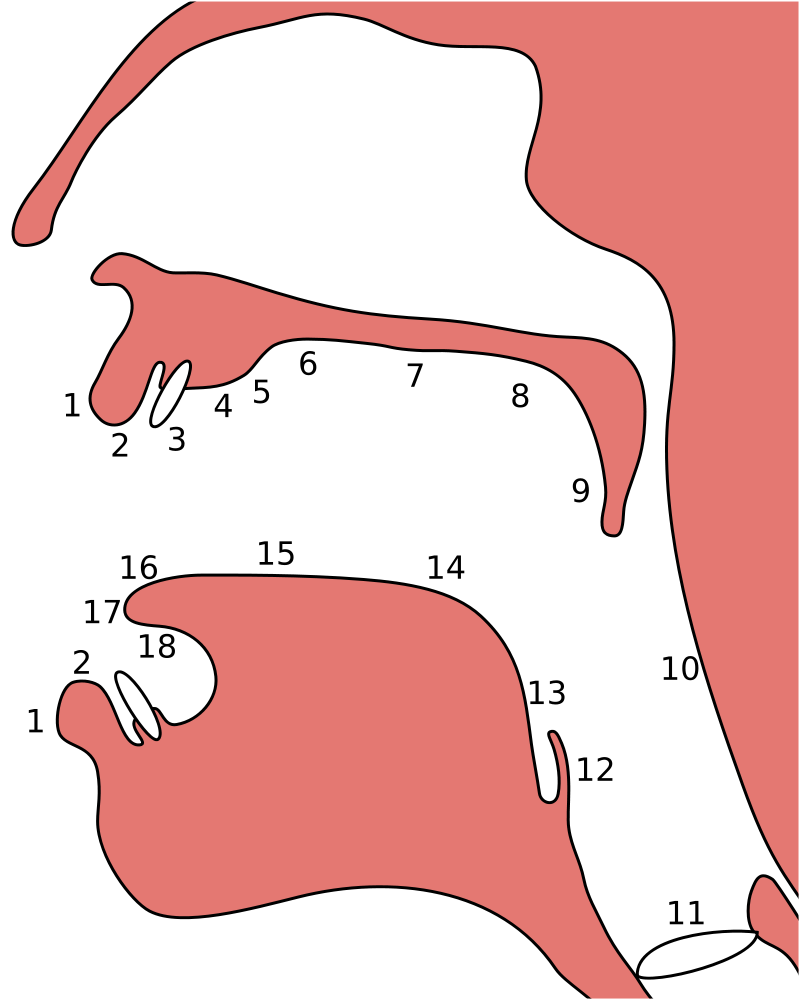
\includegraphics[width=.7\linewidth]{800px-Places_of_articulation.svg.png}
\caption{发音部位}
\end{figure}
\begin{multicols}{3}
\begin{enumerate}
\item Exo-labial
\item Endo-labial
\item Dental
\item Alveolar
\item Post-alveolar
\item Pre-palatal
\item Palatal
\item Velar
\item Uvular
\item Pharyngeal
\item Glottal
\item Epiglottal
\item Radical
\item Postero-dorsal
\item Antero-dorsal
\item Laminal
\item Apical
\item Sub-laminal
\end{enumerate}
\end{multicols}
\end{document}